%% Computer Methods and Programs in Biomedicine
%% Elsevier elsarticle class. Compile with pdfLaTeX.
%%
%% Upload this folder to Overleaf and it builds without installing anything.
%% The generated PDF is what Elsevier's system expects at submission.

\documentclass[preprint,12pt]{elsarticle}

\usepackage{graphicx}
\usepackage{booktabs}
\usepackage{amsmath}
\usepackage{url}
\usepackage{xurl}
\usepackage[hidelinks]{hyperref}

\makeatletter
\pdfstringdefDisableCommands{%
  \let\corref\@gobble
  \let\fnref\@gobble
  \let\tnoteref\@gobble
}
\makeatother

\journal{Computer Methods and Programs in Biomedicine}

\begin{document}

\begin{frontmatter}

\title{Entity-linkage failure in longitudinal health data: a detectable
defect class and an open-source validation tool}

\author[nchu,dex]{Muhammad Umer Imran\corref{cor1}}
\ead{umer@3dex.com}
\cortext[cor1]{Corresponding author.}

\address[nchu]{Clinical Medicine, Nanchang University, Nanchang, China}
\address[dex]{3Dex Inc., Irvine, CA 92617, USA}

\begin{abstract}
\textbf{Background and Objective:} A longitudinal dataset asserts that rows
sharing an identifier describe the same entity observed repeatedly over time.
Analyses depend on this assertion continuously, through lags, first differences,
trajectories, sequence models and entity-grouped cross-validation, yet it is
seldom verified. Where the assertion is false, no error is raised and
within-entity quantities lose meaning while remaining numerically plausible.
This study characterises entity-linkage failure as a detectable defect class,
provides an automated test requiring no domain knowledge, and examines whether
such defects survive conventional sanity checks.

\textbf{Methods:} Two properties distinguish a correct entity key. Certain
attributes cannot change for a real entity, and certain measures only
accumulate. Since neither property is known in advance, we quantify how much of
a table a candidate key resolves into invariants or counters, then compare this
against a null obtained by permuting entity labels within each period, which
preserves panel shape while destroying row correspondence. The method was
implemented in \texttt{paneldx}, an open-source Python package, alongside
detectors for cumulative features, target composition and the absent naive
baseline. Evaluation used 63 public longitudinal datasets, each tested with its
documented key and again after deliberate corruption. The method was then
applied to 24{,}000 physician-quarter records from a Chinese online health
community.

\textbf{Results:} Across the 63 datasets, comprising 225{,}835 rows and
32{,}503 entities, permuted keys explained zero columns in every case, and all
48 corrupted keys were rejected. Specificity was 67.4\% where any evidence
existed and 92\% on clinical panels. In the health-platform data the method
rejected the entity key used in our own previously published pipeline, which
permitted account-opening dates to change for 97.1\% of putative physicians,
and recovered the correct compound key without hints. Cumulative features
reached lag-1 autocorrelation of 0.962, and the modelling target was
reconstructible from its own predictors at held-out $R^2$ of 0.923. The defects
proved mutually concealing. Under the fabricated key a carry-forward baseline
scored $R^2$ of 0.191 and appeared uninformative, whereas under the recovered
key it scored 0.971 and outperformed the earlier model by a factor of 2.9. On
the corrected panel, patient-reported satisfaction was predictable from
behavioural signals at $R^2$ of 0.703 under leave-one-specialty-out validation.

\textbf{Conclusions:} Entity-linkage failure is a distinct and machine-detectable
defect class in longitudinal health data. Because it suppresses the naive
baseline conventionally relied upon to expose over-optimistic results, that
baseline alone offers insufficient protection, and key validity should be
established first.
\end{abstract}

\begin{keyword}
panel data \sep longitudinal data \sep data leakage \sep entity resolution \sep
reproducibility \sep health informatics
\end{keyword}

\end{frontmatter}

\section{Introduction}

Longitudinal data underpins much of health informatics. Patient trajectories,
provider performance, disease progression and health-system utilisation are all
panel structures, meaning repeated observations of the same entities across
periods. The analytical machinery applied to such data depends on a single
assumption: that rows sharing an identifier really do describe the same entity.

That assumption is rarely tested. It arrives with an extract, a join or a
spreadsheet export, and is thereafter treated as ground truth. When it fails,
the failure is silent. A grouped shift still returns a column. A recurrent
network still converges. Grouped cross-validation still partitions the data.
Every downstream number remains finite, plausible and wrong.

Kapoor and Narayanan \cite{kapoor2023} surveyed 294 papers across 17 fields and
documented leakage as a systemic driver of irreproducible machine-learning
results. Their taxonomy addresses leakage between training and test partitions,
feature-target contamination, and illegitimate feature use. It does not cover
the case in which the entity partition is itself fictitious, where rows a model
treats as one subject in fact belong to several. We argue this constitutes a
separate defect class requiring a separate test, because it is invisible to
every check in the existing taxonomy. Partitions can be scrupulously respected
while the entities defining them do not exist.

This paper makes three contributions. First, it characterises entity-linkage
failure in panel data, distinguishes it from established leakage types and
identifies its diagnostic signature. Second, it gives a null-calibrated test
that determines from data alone whether a claimed entity key is supported,
requiring no domain knowledge or user-declared schema, and implements that test
in an open-source package. Third, it demonstrates defect concealment.
Re-examining a health-platform panel from our own previously published work
\cite{prior}, we show that an invalid entity key suppresses the naive baseline
that would otherwise have exposed a weak model. The ordering of validity checks
is therefore not arbitrary.

\section{Background and related work}

Existing tooling addresses adjacent problems. LeakageDetector \cite{drosos2025}
performs static analysis over notebooks, flagging preprocessing before
splitting, overlapping partitions and multi-test issues. It inspects source code
and never examines data, so a table whose entity identifier is fabricated passes
unremarked. Julearn \cite{hamdan2024} prevents leakage by construction, wrapping
cross-validation so that preprocessing cannot cross partition boundaries. This
is prophylactic rather than diagnostic and cannot audit a dataset already in
hand.

Record linkage tools solve the converse problem. Splink \cite{linacre2022}
performs probabilistic entity resolution, creating links between records that
lack a shared identifier. Here a claimed identifier already exists and the
question is whether it is real. Linkage constructs; validation adjudicates.

Schema validators such as Great Expectations and pandera assert type, range and
nullity constraints supplied by the user. They enforce declared expectations and
cannot discover that an undeclared structural assumption has failed.

To our knowledge no existing tool tests the structural integrity of a claimed
panel from the data itself. The gap matters in health informatics, where
longitudinal extracts routinely pass through de-identification, re-indexing and
re-sorting, each of which can sever an identifier from the entity it names.

\section{Methods}

\subsection{Diagnostic signature}

A correct entity key induces structure that an incorrect key cannot. We exploit
two properties.

Attribute invariance concerns values that cannot change for a real entity, such
as a birth date, an account-opening timestamp or a permanent categorical
assignment. Under the correct key these are constant within an entity. Under an
incorrect key they vary.

Counter monotonicity concerns measures that only accumulate, such as lifetime
totals or cumulative visit counts. Under the correct key their within-entity
first differences are non-negative. Under an incorrect key they fluctuate in
both directions.

Neither property is known in advance, and requiring users to declare them would
defeat the purpose of an automated audit. We therefore measure how much of this
structure a candidate key reveals.

\subsection{Null calibration}

Structure alone is insufficient evidence, since columns with low variance appear
invariant under any labelling. Each candidate is therefore compared against a
null.

Let $E$ denote entity labels induced by a candidate key and $T$ the period
column. The null $E^{*}$ is obtained by permuting $E$ within each level of $T$.
This preserves the panel's shape exactly, retaining the same number of entities,
the same rows per period and the same marginal distributions, while destroying
correspondence between rows across periods. It is the distribution from which a
positionally fabricated key is drawn.

A column counts as evidence only where the candidate key explains it and the
null does not. For invariance we require the within-entity multi-value rate
under $E$ to fall below tolerance $\tau_{I}$ while the mean rate under $E^{*}$
exceeds $2\tau_{I}$. An analogous condition with $\tau_{M}$ governs counters. We
set $\tau_{I} = 0.02$ and $\tau_{M} = 0.05$. Both are deliberately loose, since
genuine keys collide occasionally and real columns carry corrections and
backfills.

\subsection{Share rather than count}

The verdict is driven by the proportion of columns explained,

\begin{equation}
\text{evidence\_frac} =
\frac{|\text{invariants}| + |\text{counters}|}{|\text{usable columns}|}
\end{equation}

This distinction is decisive. A key derived from row position in a table sorted
by some ranking explains the few columns determining that order and nothing
more, whereas a genuine entity key explains most of the table. Judged by
absolute count both appear to have found structure. Judged by share they
separate cleanly. In the case study below the separation is 7\% against 45\%.

Values at or above 0.40 are classified as supported, 0.15 to 0.40 as weak and
requiring inspection, and below 0.15 as unsupported.

\subsection{Invariance floor}

One further rule is required. A candidate explaining no invariants, whose
invariance rate is indistinguishable from its null, is rejected irrespective of
how many counters it explains.

The rationale is specific. Where rows are ranked by a column that grows over
time, the value at rank $i$ also grows over time. Such a key inherits
monotonicity from the sort order rather than from any entity. Counters alone
cannot support a key, since real entities always possess at least one persistent
attribute.

\subsection{Key discovery}

Where no key is supplied, all combinations of up to $k$ columns are searched,
with $k$ set to 2 by default. Individual columns are not filtered by
cardinality, because genuine keys frequently pair a coarse column with a fine
one, such as a four-valued specialty with a timestamp, and discarding the coarse
component loses the key. Only per-row-unique columns are excluded, since these
make every row its own entity.

Candidates are screened on shape before scoring, screening being substantially
cheaper. A candidate must appear at most once per period and leave sufficient
entities with sufficient observations. Survivors are ranked by explanatory power
discounted by coverage, computed as the share of columns explained multiplied by
the square root of coverage, so that a key fragmenting the panel cannot win on
cleanliness alone. Ties break toward the finer partition, since two keys may
score identically while one silently merges entities sharing a value.

\subsection{Companion detectors}

Key validation establishes whether within-entity arithmetic is meaningful. Three
further checks establish whether the resulting numbers will mislead.

Cumulative features move little between periods, so any target constructed from
them is autocorrelated by construction and a model fitted to it scores well for
restating its own inputs. Non-negative numeric columns that vary within entities
yet essentially never decrease are flagged, with lag-1 autocorrelation reported.

Target composition arises where the target is computed from columns also serving
as predictors, so that the model recovers arithmetic rather than performing
prediction. Ordinary least squares is fitted on half the rows and scored on the
held-out half. The model is deliberately linear, since the objective is not to
predict the target well but to demonstrate that no prediction was required.
Held-out $R^2$ at or above 0.99 indicates a deterministic function, and 0.90 or
above indicates substantial reconstructibility warranting investigation.

The absent naive baseline is the third check. On autocorrelated panels, carrying
the last observed value forward is frequently unbeatable, and scoring it gives
any model an honest comparator.

\subsection{Implementation}

The method is implemented in \texttt{paneldx}, a Python package depending only
on NumPy and pandas. The restriction is deliberate, since the tool is intended
to run before a modelling stack is chosen. A library interface and a
command-line interface are provided, the latter exiting non-zero when a defect
invalidating within-entity analysis is found, permitting use as a pipeline gate.
Results render to a self-contained HTML report. The package is released under
Apache-2.0, available on PyPI, and tested on Python 3.9 through 3.13.

\section{Evaluation on public longitudinal datasets}

A method demonstrated only on the dataset motivating it invites the objection
that it detects one specific bug. It was therefore evaluated across independent
public panels.

\subsection{Design}

The Rdatasets collection \cite{arel2018} of 3{,}648 datasets was screened for
genuine panel structure, requiring an identifier repeating across at least three
levels of a time column, appearing at most once per level, and leaving at least
20 entities. This yielded 63 datasets spanning econometrics, epidemiology and
clinical trials, totalling 225{,}835 rows and 32{,}503 entities.

For specificity, the documented entity key was validated as distributed. These
are published panels whose keys are correct by construction, so any rejection is
a false positive. For sensitivity, each panel was corrupted as the case-study
pipeline had been, with rows re-sorted within each period and re-linked by
position. Any acceptance is a false negative.

One methodological detail proved essential. An initial corruption sorted on an
arbitrary numeric column, and in twelve datasets that column was time-invariant,
such as years of education, baseline seizure count or route distance. Sorting on
a time-invariant column produces an identical ordering in every period, so
position $i$ maps to exactly one true entity and the key is not corrupted at
all. The apparent 81\% sensitivity of that first run was an artefact of a
corruption that did not corrupt. The procedure now selects the column with
greatest within-entity variation and verifies that positions do not map
one-to-one onto entities before a case is counted.

\subsection{Results}

\begin{table}[htbp]
\centering
\caption{Performance across 63 public longitudinal datasets.}
\label{tab:performance}
\begin{tabular}{lr}
\toprule
Metric & Value \\
\midrule
Sensitivity, corrupted keys rejected & 100.0\% (48 of 48) \\
Specificity, all datasets & 49.2\% (31 of 63) \\
Specificity, where evidence exists & 67.4\% (31 of 46) \\
Evidence obtained by a permuted key & max 0.0, mean 0.000 \\
\bottomrule
\end{tabular}
\end{table}

\begin{figure}[htbp]
\centering
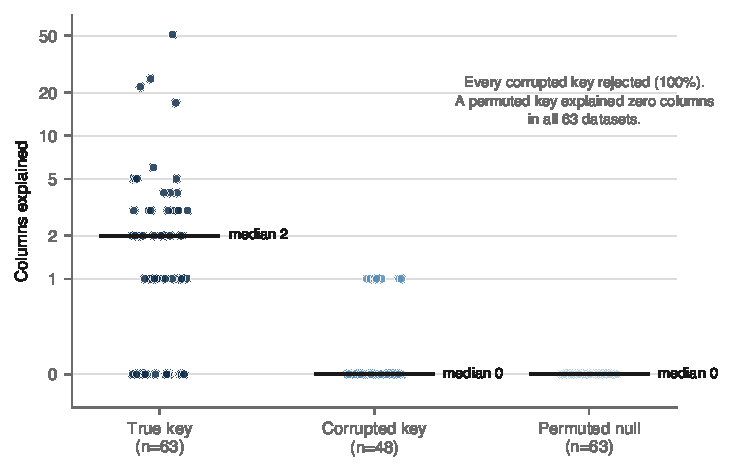
\includegraphics[width=0.85\textwidth]{../figures/figure1_null_separation.pdf}
\caption{Columns explained under the documented entity key, under a key
fabricated by re-sorting and positional linkage, and under a within-period
permutation of true labels. One point per dataset, with horizontal bars marking
medians. The vertical axis is symmetric-logarithmic so that four wide tables do
not compress the region where separation occurs.}
\label{fig:null}
\end{figure}

Null calibration proved exact. Across all 63 datasets, a key whose labels were
permuted within period explained zero columns. The separation the method relies
upon is therefore not a matter of degree, since genuine keys explain columns and
fabricated ones explain none, and every corrupted key was rejected.

Specificity requires interpretation. In 17 of 63 datasets the correct key
explained no columns, because the table contains no persistent attribute and no
accumulating counter. These are predominantly macroeconomic panels of state or
country by year, in which every column is a continuously varying economic
measure. No variant of this method can validate such a table, since the
information it relies upon is absent. Restricted to the 46 datasets where
evidence exists, specificity is 67.4\%.

\subsection{Domain dependence}

Performance separates sharply by data type.

\begin{table}[htbp]
\centering
\caption{Specificity by domain, restricted to datasets where evidence exists.}
\label{tab:domain}
\begin{tabular}{lrrr}
\toprule
Domain & $n$ & Specificity & Median columns \\
\midrule
Clinical and biomedical & 12 & 92\% & 4 \\
Economic and other & 34 & 59\% & 12 \\
\bottomrule
\end{tabular}
\end{table}

\begin{figure}[htbp]
\centering
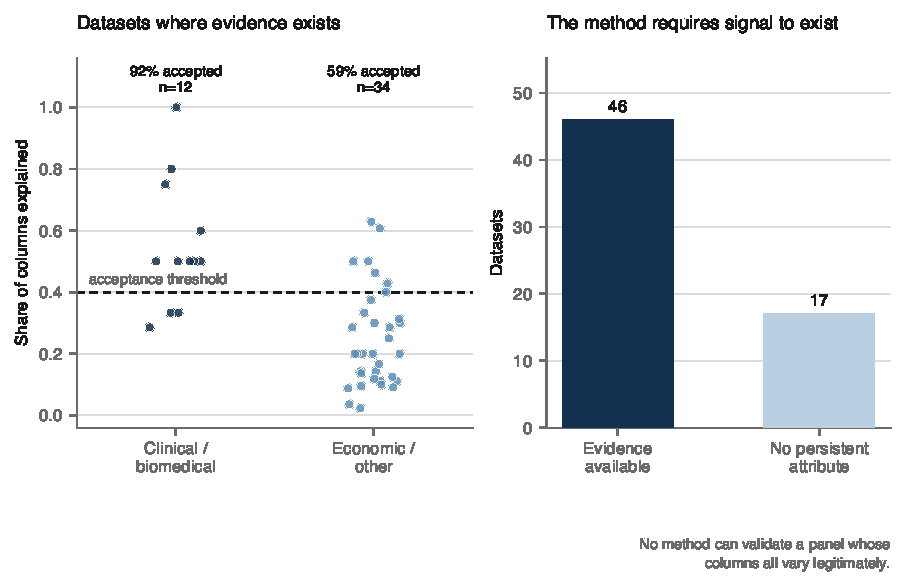
\includegraphics[width=\textwidth]{../figures/figure2_domain_dependence.pdf}
\caption{Left: share of columns explained under the true key, by domain, for the
46 datasets where evidence exists, with the dashed line marking the acceptance
threshold. Right: the 17 datasets in which no column is either persistent or
accumulating, and which therefore cannot be validated by this or any similar
method.}
\label{fig:domain}
\end{figure}

Clinical panels carry the structure the method requires, since patients have a
sex, a treatment allocation, a baseline measurement and a date of enrolment.
Wide economic panels of purely time-varying quantities do not.

This favours the intended application. The method is most reliable in the domain
where longitudinal data is most common in health informatics, and its weakness
falls in a data type where the entity key is typically a well-known geographic
identifier that no one doubts.

\subsection{Residual weakness}

Among the 15 datasets where evidence existed but the key was rejected, the
pattern is consistent. These are wide tables in which a small number of genuine
invariants is diluted by many legitimately varying columns. In one
labour-economics panel, five columns of real evidence stand against a
permuted-key baseline of zero, yet five of 42 columns falls below the 0.40
threshold.

An alternative rule thresholding the absolute count of explained columns was
tested. At a threshold of two columns it achieves 69.6\% specificity against the
share rule's 67.4\%, with sensitivity unchanged at 100\%. The improvement is too
marginal to justify changing shipped behaviour.

A more consequential problem is that the implementation reports the same verdict
for two materially different situations: a key contradicted by evidence, and a
table containing no evidence to weigh. These warrant different responses from an
analyst. Separating them by testing whether any column has cardinality low
enough to be invariant identified only 4 of the 17 cases correctly, since a
low-cardinality column may still vary within an entity. A reliable abstention
criterion remains open and is the most valuable addition the method could
receive.

\section{Case study}

\subsection{Setting and data}

We audited a modelling pipeline of our own, previously published \cite{prior}.
The dataset comprises 24{,}000 physician-quarter records across 31 columns, four
quarters and four disease areas, namely leukemia, lung cancer, breast cancer and
hepatitis, scraped from a large Chinese online health community where patients
select physicians partly on platform-displayed reputation signals. The earlier
pipeline combined a tabular transformer with a recurrent component to predict a
composite popularity index and reported a mean absolute error of 0.0942.

The data contains attributes inferred from physician photographs, which
constitute sensitive personal information under the Personal Information
Protection Law and Article 9 of the General Data Protection Regulation. It is
not redistributed, and the analysis code accepts a path to a local copy.

\subsection{Entity linkage}

The pipeline constructed its physician identifier from row position, computing
the serial number modulo the number of rows per quarter. Each quarter had been
sorted by the platform's recommendation rank before this operation, so position
$i$ denoted whichever physician ranked $i$-th in that quarter, a different
individual each period.

The method rejected this key, explaining 7\% of columns, or 2 of 30. The direct
evidence is unambiguous. Under this key, account-opening date varied for 97.1\%
of putative physicians, gender for 66.1\%, and cumulative visit counts decreased
between consecutive periods in 46.9\% of transitions.

Given no hints, blind search over all one- and two-column combinations ranked
disease area combined with account-opening time first, explaining 45\% of
columns across 4{,}210 physicians and covering 69.9\% of rows. Under this key,
counter violations fall from 46.9\% to 1.0\%, the diagnostic signature of
correct linkage. Restricting to physicians unambiguously identified and present
in all four quarters yields a corrected panel of 4{,}035 physicians across four
quarters.

Consequences for the original pipeline were total. Momentum features were
differences between unrelated physicians, the recurrent component modelled
trajectories stitched from four different people, and entity-grouped
cross-validation did not separate entities.

\subsection{Cumulative features and target composition}

Under the recovered key the tool identified cumulative counters including total
patients at lag-1 autocorrelation of 0.962, medical consultation records at
0.961 and total visits at 0.871. These are lifetime totals rather than
per-period flows, and a target constructed from them is autocorrelated by
construction, which explains why the modelling task appeared tractable.

The popularity index was defined as the mean of four standardised components,
three of which, being log visits, log gifts and inverse rank, also appeared
among the predictors. Target-composition analysis returned held-out $R^2$ of
0.923 and identified those three as the strongest contributors, recovering the
target's own definition from the data.

\subsection{Defect concealment}

The central methodological finding is that these defects concealed one another.

\begin{table}[htbp]
\centering
\caption{The same carry-forward baseline scored under each entity key.}
\label{tab:concealment}
\small
\begin{tabular}{lrrl}
\toprule
Entity key & MAE & $R^2$ & Apparent conclusion \\
\midrule
Positional, as used & 0.4717 & 0.191 & Baseline is uninformative \\
Recovered & 0.0320 & 0.971 & Baseline beats the model 2.9-fold \\
\bottomrule
\end{tabular}
\end{table}

\begin{figure}[htbp]
\centering
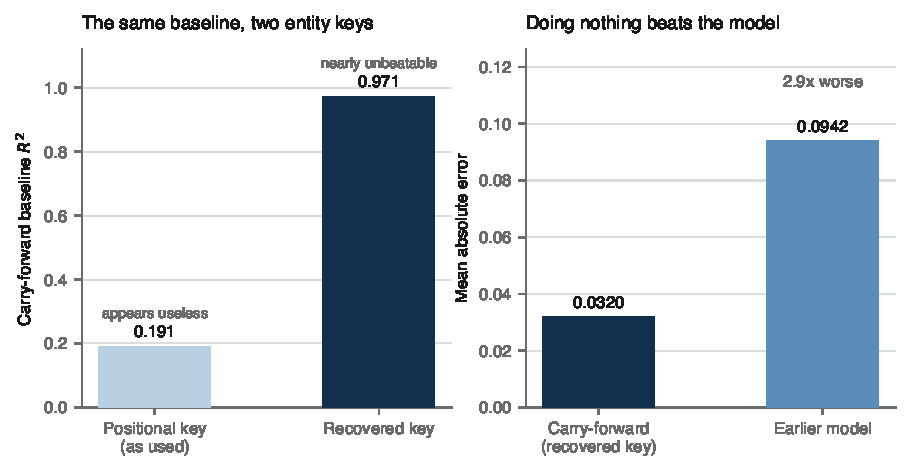
\includegraphics[width=\textwidth]{../figures/figure3_concealment.pdf}
\caption{Left: the same carry-forward baseline scored under each entity key.
Right: that baseline against the earlier model's reported error, both computed
on the recovered key.}
\label{fig:concealment}
\end{figure}

Under the fabricated key the carry-forward forecast compares unrelated
physicians and therefore performs poorly. An analyst running this standard
sanity check would conclude the baseline was uninformative and proceed with
confidence. Under the correct key the same baseline is near-unbeatable, and the
earlier model proves 2.9 times worse than doing nothing.

The implication generalises. Naive-baseline comparison is widely recommended as
protection against exactly this class of error, yet it is not robust to
entity-linkage failure, because the linkage defect disarms it. Baseline
comparison is necessary but insufficient, and key validity must be established
first. This ordering is enforced in the implementation, where the audit
establishes the key before reporting any baseline.

\subsection{What the corrected data supports}

Reanalysis of the corrected panel identifies a target the data genuinely
supports. Predicting patient-reported satisfaction from behavioural and
operational signals alone, excluding every rating-derived column, achieves $R^2$
of 0.703, with mean absolute error of 0.147 against 0.261 for a mean-only
baseline, a 44\% reduction, on 4{,}035 physicians and 26 features.

Validation used leave-one-specialty-out folds, so models were trained on three
disease areas and scored on a fourth never seen during training. Performance
therefore reflects transfer across clinical specialties rather than
within-specialty memorisation, which is both the more demanding and the more
clinically relevant criterion.

The dataset was not devoid of signal. The original formulation asked a question
its own construction had already answered.

\section{Discussion}

Entity-linkage failure is distinct from established leakage types. Existing
taxonomies assume entities exist and ask whether information crosses between
them, whereas here the entities themselves are artefacts. No amount of partition
hygiene detects this, since partitions can be perfectly respected while meaning
nothing.

The failure mode is likely under-recognised. It requires only that a
longitudinal extract be re-sorted between periods and subsequently joined by
position, an unremarkable event in any pipeline involving spreadsheet exports,
de-identification passes or re-indexing. Because it raises no error and degrades
no metric visibly, true incidence probably exceeds reported incidence
substantially.

Concealment implies ordering. The finding that a broken key suppresses the naive
baseline generalises, since any validity check computed within entities is
compromised by an invalid entity definition. Checks therefore have a dependency
order, with key validation at its root.

Self-audit proved feasible and worthwhile. This work originated in re-examining
our own published pipeline, and the defects were not detectable by inspection of
results, since reported metrics were unremarkable and internally consistent.
They became visible only when the entity assumption was tested directly.

\section{Limitations}

A supported verdict indicates that data is consistent with a key, not that the
key is correct. Domain knowledge remains authoritative.

Tolerances exist because genuine keys collide, so a key merging a small number
of entities may score comparably to a clean one. Tie-breaking toward finer
partitions mitigates this without eliminating it.

Leakage detection is linear, so a target derived from its predictors by a
non-linear rule may evade it. A high score is strong evidence of composition,
whereas a low score is not a clearance.

The implementation does not distinguish a key contradicted by evidence from a
table containing no evidence to weigh, reporting both as unsupported. This
affected 17 of 63 datasets in evaluation.

Specificity is domain-dependent, at 92\% on clinical panels against 59\% on wide
economic panels, where a few genuine invariants are diluted by many legitimately
varying columns.

The method requires at least two periods and sufficient entities to estimate
rates. Tables consisting entirely of volatile measurements cannot be validated
by this approach.

\section{Conclusion}

Entity-linkage failure is a distinct, consequential and machine-detectable
defect class in longitudinal health data. It invalidates within-entity analysis
while producing no error, and it suppresses the naive-baseline comparison
conventionally relied upon to detect over-optimistic results. This study
characterises the defect, provides a null-calibrated test requiring no domain
knowledge, and demonstrates on health-platform data that a model previously
believed adequate was 2.9 times worse than carrying the last value forward.

Validation of the entity key should precede any within-entity analysis of panel
data, and naive baselines should be reported only after that validation has
passed.

\section*{CRediT authorship contribution statement}

\sloppy
\textbf{Muhammad Umer Imran:} Conceptualization, Methodology, Software, Formal
analysis, Investigation, Data curation, Writing (original draft), Writing
(review and editing), Visualization.

\section*{Declaration of competing interest}

The author declares no known competing financial interests or personal
relationships that could have appeared to influence the work reported in this
paper.

\section*{Data availability}

\sloppy

The software is available at \url{https://github.com/stemmatics/paneldx} under
Apache-2.0, installable from PyPI as \texttt{paneldx}, and archived at
\url{https://doi.org/10.5281/zenodo.22086706}. Analysis code reproducing every
quantitative claim, together with the intermediate results underlying every
figure and table, is available at
\url{https://github.com/stemmatics/paneldx-paper} and archived at
\url{https://doi.org/10.5281/zenodo.22086703}. The 63 evaluation datasets are
public and retrievable from the Rdatasets collection \cite{arel2018}. The
physician panel is not redistributed, since it contains attributes inferred from
photographs of identifiable individuals; the analysis code accepts a path to a
local copy.

\section*{Funding}

This research received no specific grant from funding agencies in the public,
commercial or not-for-profit sectors.

\begin{thebibliography}{9}

\bibitem{kapoor2023}
S.~Kapoor, A.~Narayanan,
Leakage and the reproducibility crisis in machine-learning-based science,
Patterns 4 (2023) 100804.
\newblock \url{https://doi.org/10.1016/j.patter.2023.100804}

\bibitem{drosos2025}
I.~Drosos, T.~Barik, P.~J. Guo, R.~DeLine, S.~Gulwani,
LeakageDetector: an open source data leakage analysis tool in machine learning
pipelines, arXiv:2503.14723 (2025).

\bibitem{hamdan2024}
S.~Hamdan, B.~C. Love, G.~G. von Polier, S.~Weis, H.~Schwender, S.~B. Eickhoff,
et~al.,
Julearn: an easy-to-use library for leakage-free evaluation and inspection of
ML models, Gigabyte 2024 (2024) gigabyte113.
\newblock \url{https://doi.org/10.46471/gigabyte.113}

\bibitem{linacre2022}
R.~Linacre, S.~Lindsay, T.~Manassis, Z.~Slade, T.~Hepworth,
Splink: free software for probabilistic record linkage at scale,
International Journal of Population Data Science 7 (2022) 1794.
\newblock \url{https://doi.org/10.23889/ijpds.v7i3.1794}

\bibitem{arel2018}
V.~Arel-Bundock, N.~Enevoldsen, C.~J. Yetman,
Rdatasets: an archive of datasets distributed with R,
Journal of Open Source Software 3 (2018) 892.
\newblock \url{https://doi.org/10.21105/joss.00892}

\bibitem{prior}
M.~U. Imran, S.~J. Raza, S.~Yiying, S.~N.~A. Shah, S.~D.~A. Naqvi, A.~Rehman,
A multidimensional, transformer-based framework for predicting physician
popularity on online health platforms,
Haya: The Saudi Journal of Life Sciences 10 (2025) 773--790.
\newblock \url{https://doi.org/10.36348/sjls.2025.v10i11.009}

\end{thebibliography}

\end{document}
